\chapter{序論}
\label{introduction}

本研究では、惑星規模の分散システムのためのステージング環境の設計と構築を行う。

本章では、まず初めに惑星規模の分散システムを定義し、本研究の背景である惑星規模の分散システムの発達とシステムのステージング環境について概説する。
次に、本研究の課題を明らかにした上で、目的を明確化し、目的を達するための仮説を示す。
最後に仮説を裏付けるための提案手法を示し、本研究の概要を示す。

\section{本研究の背景}
\label{introduction:background}

本節では、本研究の背景について述べる。

まず初めに、本研究が対象とする惑星規模の分散システムとステージング環境について概説する。
惑星規模の分散システムの定義にあたって、比較しやすくするため、別のシステムモデルであるモノリスと分散システムについても述べる。
次に、惑星規模の分散システムの発達について述べ、その後に惑星規模の分散システムに求められるステージング環境について説明する。

\subsection{惑星規模の分散システム}

本研究における惑星規模の分散システムを定義する前に、惑星規模の分散システムとは別のシステムモデルであるモノリスと分散システムについて概説する。

まず、モノリスとはモノシリックなシステムを指し、本研究では単一のコンポーネントで構成されるシステムと認識する。

次に、分散システムはモノリスとは対称的に複数のコンポーネントが組み合わさって動作するシステムである。
分散システムでは、複数の独立したコンポーネントが協調動作することによってシステム全体が成り立っている。

最後に、惑星規模の分散システムは、分散システムの中でも世界中に地理的に分散したコンピュータによって構成されるものを指す。
システム全体が特定の箇所に収まらず、世界中のあらゆる箇所のコンピュータが協調動作することによってシステム全体が機能する点が特徴的である。
具体的には、ブロックチェーン~\cite{Bitcoin}が惑星規模の分散システムに属する。
惑星規模の分散システムを支える技術としては、P2Pが挙げられる。
P2Pは``Peer to Peer''の略であり、コンピュータ同士が対等な関係を築き協調動作する、中央集権的なサーバを必要としないシステムモデルである。
クライアントサーバモデルのシステムのように、システム内に明確な役割分担と主従関係のあるシステムとは対照的である。
クライアントサーバモデルでは,通信において常にクライアント対サーバで一対一の関係が成り立つ.
クライアントはサーバに対してリクエストを送り,リクエストを受け取ったサーバは特定の処理に基づいてクライアントに対しレスポンスを返す.
対してブロックチェーンのようなP2Pのシステムでは,参加するコンピュータの役割は状況に応じて柔軟に変化する.
時にクライアントとして他のコンピュータに対して要求し,時に他のコンピュータからの要求に対して応答する.
クライアントサーバモデルに比べて,耐障害性・冗長性・可用性において優れているのが特徴的である.

\subsection{惑星規模の分散システムの発達}

2000年代初頭,Winny~\cite{Winny}やGnutella~\cite{Gnutella}といった惑星規模の分散システムが頭角を現した.
どちらのサービスもP2P技術を基盤としており、それまでシステムモデルとして一般的であったクライアントサーバモデルとは異なる形態を採用したことで注目が集まった。
P2P技術が研究分野で取り上げられる頻度も多くなり、サービスとしても今後一層幅を広げていくと思われたが、クライアントサーバモデルに置き換わるまでの隆盛はなく後退していった.
しかし,2008年にSatoshi NakamotoによりBitcoinのために開発されたブロックチェーン技術が登場することによって,再度P2P技術が脚光を浴びるようになり,開発や研究の勢いが再び盛んになってきている.

\subsection{ステージング環境}

ステージング環境とは,本番環境での運用をする前に実際の環境を想定してシステム全体のテストを行うための環境である.
開発者が実際に開発を行う開発環境と実運用する本番環境では,環境の差異から動作の違いが生じ,手元で正常に動作していたものが本番環境に反映した途端動作しなくなるといった事象が度々発生する.
そのような事態を防ぐために開発環境と本番環境の間に,本番環境を想定したステージング環境を構築し,本番環境へのデプロイ前にステージング環境にて動作を確認することで予想外の障害が発生するリスクを抑えることができる.
惑星規模の分散システムにおいても、実運用での不具合や軽微なバグを早期に発見するためにステージング環境が必要である。
モノリスの場合、システムは単一のコンポーネントで構成され、システムを構成するサーバの配置は開発者が任意に決定できる。
よって、本番環境と同じ構成をオンプレ環境もしくはクラウド環境を用いて構築し、システムに対して任意の入力をした際に期待する動作がされるかどうかを確認すればよい。
一方、分散システムの場合もモノリスと同じくサーバの配置は開発者が指定できるため、ステージング環境の構築は比較的容易である。
しかし、分散システムは複数のコンポーネントから構成されるため、各コンポーネントのテストに加え、すべてのコンポーネントを通したシステム全体でのテストを行う必要がある。
最後に、惑星規模の分散システムのテストはモノリスや分散システムに比べて難易度が高くなる。
何故なら、惑星規模の分散システムにおいて、システムを構成するコンピュータは世界中に地理的に分散しており、開発者がシステム全体の構成を固定できないからである。
システムには世界中の至る場所からコンピュータが参加し、システム全体も常にスケーリングする可能性がある。
惑星規模の分散システムのステージング環境の構築をする場合、地理的な場所を指定し分散させてサーバを配置する必要がある。


\begin{figure}[htbp]
  \begin{center}
    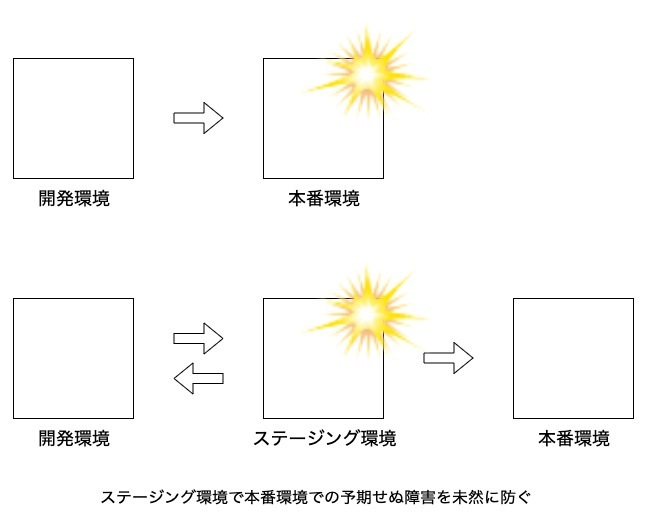
\includegraphics[width=0.8\textwidth]{./figures/staging.jpg}
    \caption{ステージング環境}
  \end{center}
\end{figure}

\section{本研究の課題と目的}
\label{introduction:issue-aim}

本節では、本研究の課題と目的を述べる。

まず、~\ref{introduction:background}章で述べた本研究の背景を元に、惑星規模の分散システムのステージング環境における課題を示す。
その上で本研究の目的を明確にする。

\subsection{本研究の課題}
\label{introduction:issue-aim:issue}

本研究では、惑星規模の分散システムのためのステージング環境の構築が困難であり、構築手法が未だ整っていないことを課題とする。

モノリスや分散システムといった開発者がサーバの配置を任意で決めることができ、システム全体の構成を固定化できるサービスの場合、ステージング環境の構築は比較的容易であると述べた。
対して惑星規模の分散システムの場合、開発者がシステム内のサーバの配置や数といった構成を固定化することは出来ず、システムは常に変化する可能性がある。
よって、惑星規模の分散システムのステージング環境においては、本番での実運用を考えて実際に地理的に離れた場所に分散してサーバを設置する必要がある。

地理的に離れた場所にサーバを用意する手段のひとつとして、クラウド環境の利用が考えられる。
クラウド環境では、リージョンという属性があり、地理的な場所を指す。
リージョンを指定することで地理的に離れた場所にサーバを設置することが可能である。
しかし、本研究ではクラウドサービスを用いた手法では惑星規模の分散システムのテストには不十分であると考えた。
惑星規模の分散システムでは、すべてのユーザがクラウド環境を使用する訳ではなく、オンプレ環境を用いることもある。
クラウド環境では、ネットワークの帯域幅が十分に設けられていたり、サーバはデータセンターないで管理されており強制終了などの予期せぬ事態も起こりにくい。
本番環境をより厳密に想定するのであれば、クラウドサービスを使うよりもオンプレ環境を用いたステージング環境の構築をした方が好ましいと考えた。
さらに、オンプレ環境を用いた場合、クラウドサービスを使用するよりもより自由にサーバの配置を設定することが可能である。

ここで、サーバを地理的に分散配置した場合、システム全体を統合管理することが困難であることが課題となる。
物理的に離れたすべてのサーバに対し同じオペレーションをするには、各地点のオペレータがアプリのインストールやアップデートの作業を手作業で行う必要がある。
システム全体に修正が加えられる度に、オペレータ同士での作業の把握や手作業を挟むことになり、システムのテストを行うまでに多くの時間が掛かってしまう。

\subsection{本研究の目的}
\label{introduction:issue-aim:aim}

本研究では,惑星規模の分散システムのためのステージング環境の構築手法を提案することを目的とする.

\section{本研究の仮説}
\label{introduction:hypothesis}

~\ref{introduction:issue-aim:issue}で述べた課題を解決するためには,地理的に分散したサーバを統合管理することで,ステージング環境での変更に対し柔軟かつ迅速に対応する必要があると考えた.

地理的に分散したサーバを統合管理するためには,
\begin{itemize}
  \item ステージング環境に含まれるサーバ同士が,お互いに通信可能な状態であること
  \item ある特定の地点から全てのサーバに対して操作が可能であること
\end{itemize}
の二点を満たさなければならない.

本研究では,上記の必要要件を満たすことで~\ref{introduction:issue-aim:issue}で述べた課題点を解決し,
~\ref{introduction:issue-aim:aim}で述べた惑星規模の分散システムのためのステージング環境の構築手法の提案を達成できると考えた.

\section{本研究の手法}
\label{introduction:proposal}

本研究では,~\ref{introduction:hypothesis}で述べた必要要件を満たすため,OpenVPNとKubernetesを用いる.

まず,Kubernetesはコンテナオーケストレーションツールであり,コンテナ化されたアプリケーションのデプロイやスケーリングを自動化し,統合管理するためのシステムである.
Kubernetesでは複数のサーバでクラスタを構成しており,クラスタ化には各サーバがお互いにIPレベルで疎通可能な状態になければならない.
よって,Kubernetesは単一のデータセンター内での使用に適している一方,複数のデータセンターを跨がった構成での使用には適していない.

そこで,地理的に分散したサーバ間を結ぶOpenVPNオーバーレイネットワークを構築することで,各サーバがお互いにIP Reachableな状態にする.
OpenVPNとは,VPNネットワークの構築をソフトウェアで実現するために開発されたオープンソースソフトウェアである.

本研究では,OpenVPNとKubernetesを組み合わせ,地理的に分散した拠点間で形成したOpenVPNオーバーレイネットワーク上でKubernetesクラスタを構築した.
別々のセグメントに位置するノードを用いてKubernetesクラスタを構築し,コンテナ化したアプリケーションをクラスタ上にデプロイできていることを確認し,
本システムの課題点を解決できているか推定することで要件を満たせることを確認した.

\section{本論文の構成}
\label{introduction:structure}

本論文における以降の構成は次の通りである.

~\ref{background}章では,惑星規模の分散システムとそのテストを行うためのステージング環境について概説した上で、それに伴う課題点について議論し,本研究の背景を明確化する.
~\ref{issue}章では,本研究で着目する問題を解決するための要件,仮説と手法について説明する.
~\ref{implementation}章では,本研究で提案するステージング環境の構築方法について述べる。
~\ref{evaluation}章では,\ref{issue}章で求められた課題に対しての評価を行い,考察する.
~\ref{conclusion}章では,本研究のまとめと今後の課題についてまとめる.

%%% Local Variables:
%%% mode: japanese-latex
%%% TeX-master: "../thesis"
%%% End:
